% Compile with: pdflatex lecture_30_31.tex
% Requires: amsmath, amssymb, amsthm, stmaryrd, mathtools, xcolor, mdframed,
%           enumitem, hyperref, pagecolor, microtype, tikz

\documentclass[11pt]{article}
\usepackage[margin=1in]{geometry}
\usepackage{amsmath, amssymb, amsthm}
\usepackage{stmaryrd}
\usepackage{mathtools}
\usepackage{xcolor}
\usepackage{mdframed}
\usepackage{enumitem}
\usepackage{hyperref}
\usepackage{pagecolor}
\usepackage[protrusion=true,expansion=false]{microtype}
\usepackage{tikz}
\usetikzlibrary{arrows.meta, positioning, shapes.geometric}

% ----- Colour palette -----
\definecolor{cream}{HTML}{FFFDF5}
\definecolor{defblue}{HTML}{1A4A7A}
\definecolor{thmgreen}{HTML}{1A5C3A}
\definecolor{warnAmber}{HTML}{7A4A00}
\definecolor{dangerRed}{HTML}{7A1A1A}
\definecolor{boxbluebg}{HTML}{EBF3FB}
\definecolor{boxgreenbg}{HTML}{EBF7EF}
\definecolor{boxamberbg}{HTML}{FDF5E6}
\definecolor{boxredbg}{HTML}{FBEBEB}
\pagecolor{cream}

% ----- Theorem styles -----
\newtheoremstyle{defstyle}{8pt}{8pt}{\normalfont}{0pt}{\bfseries\color{defblue}}{.}{0.5em}{}
\newtheoremstyle{thmstyle}{8pt}{8pt}{\normalfont}{0pt}{\bfseries\color{thmgreen}}{.}{0.5em}{}
\newtheoremstyle{notstyle}{8pt}{8pt}{\normalfont}{0pt}{\bfseries\color{warnAmber}}{.}{0.5em}{}
\newtheoremstyle{cautionstyle}{8pt}{8pt}{\normalfont}{0pt}{\bfseries\color{dangerRed}}{.}{0.5em}{}

\theoremstyle{defstyle}
\newtheorem{definition}{Definition}[section]

\theoremstyle{thmstyle}
\newtheorem{theorem}{Theorem}[section]
\newtheorem{corollary}[theorem]{Corollary}
\newtheorem{lemma}[theorem]{Lemma}

\theoremstyle{notstyle}
\newtheorem*{remark}{Remark}
\newtheorem*{example}{Example}

\theoremstyle{cautionstyle}
\newtheorem*{caution}{Caution}

% ----- Boxes -----
\newmdenv[
  backgroundcolor=boxbluebg, linecolor=defblue, linewidth=2pt,
  topline=false, rightline=false, bottomline=false,
  innerleftmargin=10pt, innerrightmargin=10pt,
  innertopmargin=6pt, innerbottommargin=6pt,
  skipabove=8pt, skipbelow=8pt
]{defbox}

\newmdenv[
  backgroundcolor=boxgreenbg, linecolor=thmgreen, linewidth=2pt,
  topline=false, rightline=false, bottomline=false,
  innerleftmargin=10pt, innerrightmargin=10pt,
  innertopmargin=6pt, innerbottommargin=6pt,
  skipabove=8pt, skipbelow=8pt
]{thmbox}

\newmdenv[
  backgroundcolor=boxamberbg, linecolor=warnAmber, linewidth=2pt,
  topline=false, rightline=false, bottomline=false,
  innerleftmargin=10pt, innerrightmargin=10pt,
  innertopmargin=6pt, innerbottommargin=6pt,
  skipabove=8pt, skipbelow=8pt
]{notebox}

\newmdenv[
  backgroundcolor=boxredbg, linecolor=dangerRed, linewidth=2pt,
  topline=false, rightline=false, bottomline=false,
  innerleftmargin=10pt, innerrightmargin=10pt,
  innertopmargin=6pt, innerbottommargin=6pt,
  skipabove=8pt, skipbelow=8pt
]{cautionbox}

% ----- Macros -----
\newcommand{\Z}{\mathbb{Z}}
\newcommand{\N}{\mathbb{N}}
\newcommand{\R}{\mathbb{R}}
\newcommand{\hcount}[1]{\bigl|\{y \in A \mid (#1, y) \in H\}\bigr|}

\begin{document}

\begin{center}
  {\Large\bfseries Lectures 30 \& 31 --- The Handshake Theorem}\\[4pt]
  {\normalsize CS 173: Discrete Structures \quad$\cdot$\quad Pigeonhole in Action}\\[2pt]
  {\small\color{gray} University of Illinois at Urbana-Champaign}
\end{center}
\vspace{1em}\hrule\vspace{1.5em}

\section{The claim}

These two lectures together give a fully worked application of the
pigeonhole principle. The result is a classic combinatorial fact about
social gatherings, but the real lesson is the \emph{technique}: encode
an everyday situation as a set, a relation, and a function, and let
cardinality do the work.

\begin{thmbox}
\begin{theorem}[Handshake Theorem]
Any room with at least two people contains two distinct people who have
shaken the same number of people's hands as each other.
\end{theorem}
\end{thmbox}

\begin{notebox}
\begin{remark}
The statement says nothing about which people, nor about the actual number
of handshakes that have happened. It is a pure existence claim: among any
group of $\geq 2$ people, the function ``how many hands has this person
shaken?'' must repeat a value.
\end{remark}
\end{notebox}

\section{Setting up the formal model (Lecture 30)}

We translate the informal statement into objects we can reason about.
Fix a number of people $n \geq 2$, and treat handshakes as a symmetric
relation on the set of people.

\subsection*{The room and the handshake relation}

\begin{defbox}
\begin{definition}[The room]
Let $n \in \N$ with $n \geq 2$. Define
\[
  A = \{z \in \N \mid z < n\},
\]
representing the set of all people in the room. Note that $|A| = n$.
\end{definition}
\end{defbox}

\begin{defbox}
\begin{definition}[The handshake relation]
Let
\[
  H = \{(x,y) \in A \times A \mid x \text{ has shaken hands with } y\}.
\]
Handshakes are symmetric: for all $x, y \in A$,
\[
  (x,y) \in H \;\Longleftrightarrow\; (y,x) \in H.
\]
\end{definition}
\end{defbox}

\begin{notebox}
\begin{remark}
We do not assume anything else about $H$ --- people may or may not have
shaken hands, and we do not assume the relation is irreflexive (in
practice nobody ``shakes their own hand''; the proof works either way).
The only structural property we use is symmetry.
\end{remark}
\end{notebox}

\subsection*{Actual and possible handshake counts}

\begin{defbox}
\begin{definition}[The set of actual counts]
Let
\[
  B = \Bigl\{\, \hcount{x} \;\Big|\; x \in A \,\Bigr\}.
\]
That is, $B$ is the set of \emph{actual} handshake counts that occur in
the room: for each person $x$, count how many people $x$ has shaken
hands with, and collect all such values.
\end{definition}
\end{defbox}

\begin{defbox}
\begin{definition}[The set of possible counts]
Let
\[
  D = \{z \in \N \mid z < n\},
\]
representing the set of \emph{possible} handshake counts. Note
$|D| = n$.
\end{definition}
\end{defbox}

\begin{notebox}
\begin{remark}
$A$ and $D$ are the \emph{same} set as bare sets of natural numbers
($\{0, 1, \ldots, n-1\}$), but they play different roles: $A$ indexes
people, $D$ indexes possible counts. We always have $B \subseteq D$,
since nobody can shake more than $n - 1$ other people's hands.
\end{remark}
\end{notebox}

\subsection*{The handshake-count function}

\begin{defbox}
\begin{definition}[Handshake count]
Define $f \colon A \to B$ by
\[
  f(p) \;\coloneqq\; \hcount{p}
        \;=\; \text{the \# of other people's hands that } p \text{ has shaken}.
\]
\end{definition}
\end{defbox}

\section{A small example}

\begin{notebox}
\begin{example}
Suppose $n = 5$, so $A = \{0, 1, 2, 3, 4\}$, with handshakes
\[
  H = \{(0,1),\, (1,0),\, (1,2),\, (2,1),\, \ldots\}.
\]
The handshake-count function $f$ might assign
\[
  f(0) = 2,\quad f(1) = 4,\quad f(2) = 1,\quad f(3) = 1,\quad f(4) = 2,
\]
giving the set $B = \{1, 2, 4\}$. Here $|A| = 5$ but $|B| = 3$, so $f$
is forced to repeat: indeed $f(0) = f(4)$ and $f(2) = f(3)$.
\end{example}
\end{notebox}

\begin{center}
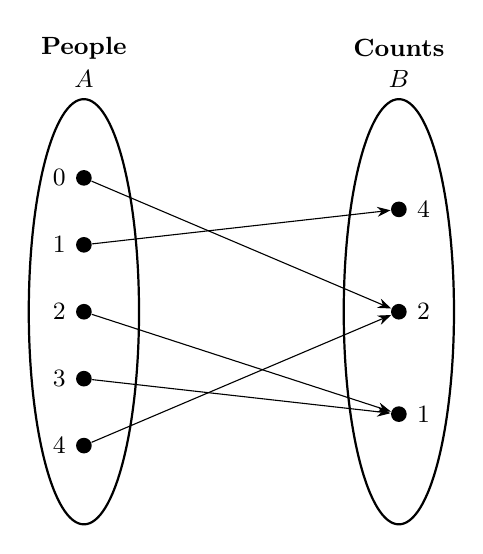
\begin{tikzpicture}[
    >=Stealth,
    dot/.style={circle, fill, inner sep=2pt},
    every node/.style={font=\small}
  ]
  % Set A
  \draw[thick] (0, 0.5) ellipse (0.7cm and 2.7cm);
  \node at (0, 3.45) {$A$};
  \node[font=\bfseries\small] at (0, 3.85) {People};

  \node[dot, label=left:{$0$}]  (a0) at (0,  2.2) {};
  \node[dot, label=left:{$1$}]  (a1) at (0,  1.35) {};
  \node[dot, label=left:{$2$}]  (a2) at (0,  0.5) {};
  \node[dot, label=left:{$3$}]  (a3) at (0, -0.35) {};
  \node[dot, label=left:{$4$}]  (a4) at (0, -1.2) {};

  % Set B
  \draw[thick] (4, 0.5) ellipse (0.7cm and 2.7cm);
  \node at (4, 3.45) {$B$};
  \node[font=\bfseries\small] at (4, 3.85) {Counts};

  \node[dot, label=right:{$4$}]  (b4) at (4,  1.8) {};
  \node[dot, label=right:{$2$}]  (b2) at (4,  0.5) {};
  \node[dot, label=right:{$1$}]  (b1) at (4, -0.8) {};

  % Arrows
  \draw[->] (a0) -- (b2);
  \draw[->] (a1) -- (b4);
  \draw[->] (a2) -- (b1);
  \draw[->] (a3) -- (b1);
  \draw[->] (a4) -- (b2);
\end{tikzpicture}
\end{center}

\begin{notebox}
\begin{remark}
The diagram makes the collision visible: persons $0$ and $4$ both map to
$2$, and persons $2$ and $3$ both map to $1$. The theorem says this kind
of collision is unavoidable --- not just here, but in \emph{every} room
of $\geq 2$ people. Lecture 31 proves this by case analysis on whether
anyone has shaken zero hands.
\end{remark}
\end{notebox}

\section{The proof by cases (Lecture 31)}

The strategy is to show $|B| < |A|$, then quote pigeonhole. The bound on
$|B|$ comes from a case split: either everyone has shaken at least one
hand, or someone has shaken zero hands. Both cases give $|B| \leq n - 1$,
but for different reasons.

We use one auxiliary fact throughout.

\begin{notebox}
\begin{remark}[Equal-size finite subset]
If $X_1, X_2$ are finite sets with $X_1 \subseteq X_2$ and
$|X_1| = |X_2|$, then $X_1 = X_2$. (A finite set cannot be a strict
subset of another set with the same size.)
\end{remark}
\end{notebox}

\begin{thmbox}
\begin{lemma}[Codomain bound]
With the setup above, $|B| \leq n - 1$.
\end{lemma}
\begin{proof}
We split on whether $0 \in B$.

\medskip
\noindent\textbf{Case 1: everyone has shaken at least one hand.}
Suppose $(\forall a \in A)(f(a) \geq 1)$. Then no person has handshake
count $0$, so $0 \notin B$. Since $B \subseteq D$, this gives
$B \subseteq D \setminus \{0\}$, so
\[
  |B| \;\leq\; |D| - 1 \;=\; n - 1.
\]

\medskip
\noindent\textbf{Case 2: someone has shaken zero hands.}
Suppose $(\exists a \in A)(f(a) = 0)$, so fix $p \in A$ with $f(p) = 0$.
We show $n - 1 \notin B$ by contradiction.

\smallskip
\noindent\emph{Assume, towards a contradiction, that $n - 1 \in B$.}
Then there exists $q \in A$ with $\hcount{q} = n - 1$.

\smallskip
\noindent\emph{Step 1: $q$ has shaken everyone else's hand.} Since $q$
does not shake their own hand,
\[
  \{y \in A \mid (q,y) \in H\} \;\subseteq\; A \setminus \{q\}.
\]
Both sides are finite of size $n - 1$, so by the equal-size finite
subset lemma,
\[
  \{y \in A \mid (q,y) \in H\} \;=\; A \setminus \{q\}.
\]

\medskip
\noindent\emph{Step 2: $p \neq q$.} If $p = q$ then
$f(p) = f(q) = n - 1$, but $f(p) = 0$ and $n \geq 2$ gives
$n - 1 \neq 0$. Hence $p \neq q$.

\medskip
\noindent\emph{Step 3: derive the contradiction.} From $p \in A$ and
$p \neq q$ we get $p \in A \setminus \{q\}$, and by Step~1
\[
  p \in \{y \in A \mid (q, y) \in H\},
\]
so $(q, p) \in H$. By symmetry of $H$, $(p, q) \in H$, hence
$q \in \{y \in A \mid (p, y) \in H\}$. Therefore
\[
  f(p) \;=\; \hcount{p} \;\geq\; 1,
\]
contradicting $f(p) = 0$. \quad\lightning

\medskip
\noindent So $n - 1 \notin B$, giving $B \subseteq D \setminus \{n-1\}$
and
\[
  |B| \;\leq\; |D| - 1 \;=\; n - 1.
\]

\medskip
In both cases, $|B| \leq n - 1$.
\end{proof}
\end{thmbox}

\begin{notebox}
\begin{remark}
The two cases knock out different elements of $D$. In Case~1 the missing
value is $0$; in Case~2 it is $n - 1$. The single fact
$\{0, n-1\} \not\subseteq B$ ties them together: the values $0$ and
$n - 1$ cannot both occur as handshake counts in the same room.
\end{remark}
\end{notebox}

\subsection*{Finishing with pigeonhole}

\begin{proof}[Proof of the Handshake Theorem]
Let $n \in \N$ with $n \geq 2$, and adopt the setup of \S2: $A$ is the
set of $n$ people, $H$ the symmetric handshake relation, and
$f \colon A \to B$ the handshake-count function. By the Codomain Bound
Lemma, we know $|B| < |A|$. Therefore, by the Pigeonhole Theorem, $f$
is not injective. This means there exist $p_1, p_2 \in A$ such that
\[
  p_1 \neq p_2 \quad\text{and}\quad f(p_1) = f(p_2).
\]
These two distinct people have shaken the same number of hands. \qedhere
\end{proof}

\begin{notebox}
\begin{remark}[Empty-set characterisation]
For any set $X$, $|X| = 0 \iff X = \emptyset$. This is the bridge
between cardinality talk ($f(p) = 0$) and set talk
($\{y \in A \mid (p,y) \in H\} = \emptyset$) used silently throughout
Case 2.
\end{remark}
\end{notebox}

\begin{cautionbox}
\begin{caution}
The theorem requires $n \geq 2$. With $n = 1$ there is only one person
in the room, so ``two distinct people'' does not exist and the statement
is vacuously false rather than vacuously true. The proof also breaks at
$n = 1$: the Case-2 argument relies on $n - 1 = 0$ being a possible
codomain value, but the only person in the room would simultaneously
need to satisfy $f(p) = 0$ and have shaken everyone else's hand --- a
contradiction generated by the empty ``everyone else.''
\end{caution}
\end{cautionbox}

\section{Summary}

\begin{enumerate}[leftmargin=2em]
  \item \textbf{Model the situation.} People form a set $A$ with $|A| = n$,
    and handshakes form a symmetric relation $H \subseteq A \times A$.
  \item \textbf{Build the right function.} The handshake-count map
    $f \colon A \to B$ has actual codomain $B \subseteq D = \{0, 1, \ldots, n-1\}$.
  \item \textbf{Bound the codomain by cases.}
    \begin{itemize}[leftmargin=1.5em, itemsep=2pt]
      \item If everyone has shaken $\geq 1$ hands, then $0 \notin B$.
      \item If someone has shaken $0$ hands, then $n - 1 \notin B$
        (otherwise the universal hand-shaker contradicts the zero-shaker
        via symmetry).
    \end{itemize}
    Either way, $|B| \leq n - 1$.
  \item \textbf{Apply pigeonhole.} Since $|A| > |B|$, no function
    $A \to B$ --- and in particular $f$ --- can be injective, so two
    distinct people share a handshake count.
\end{enumerate}

\begin{notebox}
\begin{remark}[Looking ahead]
This is a template. Many ``in any group of $n$ objects, two must share
a property'' results follow the same pattern: build a counting function
into a codomain that is provably smaller than the domain, then quote
pigeonhole. The work is almost always in shrinking the codomain by one
--- finding the structural reason a value cannot occur.
\end{remark}
\end{notebox}

\end{document}